\section{Multi-output Gaussian Process model via Neural network}

\begin{figure}[!htb]
    \centering
    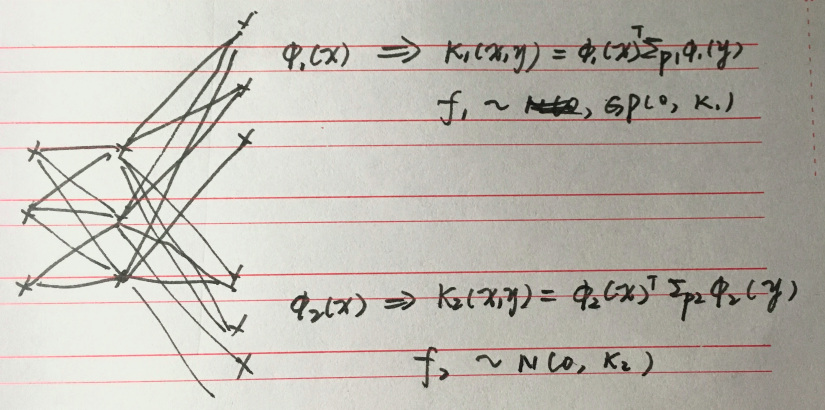
\includegraphics[width=\columnwidth]{./img/NN-MOGP.png}
    \caption{Architechure of the multi-output Gaussian process model}
    \label{fig:MONNGP}
\end{figure}

We have shown that a GP can be constructed from a neural network with finite hidden units in the last layer, in this second, we show how we can model the nonlinear correlation between tasks and define a multi-output Gaussian process model from neural network. 

Suppose we have $Q$ tasks, firstly, a neural network is used to define a \emph{shared feature map} $\phi_s : R^D \rightarrow R^{M_s}$, then, for each task $i, i \in \{1,~\dots~,Q\}$, the shared feature $\phi_s(\bm{x})$ is followed by a neural network that defines a \emph{task-specific feature map} $\phi_i : R^{M_s} \rightarrow R^{M_i}$. We assume the $i$-th latent function $f_i(\bm{x})$ follows a GP distribution $f_i \sim \mathcal{GP}(0, k_i)$ with kernel function $k_i(\bm{x}, \bm{y})$ defined as:

\begin{equation}
    \label{eq:mo_kernel}
    \left\{
    \begin{array}{lll}
        y_i                 &=&    f_i(\bm{x}) + \epsilon_i  \\
        f_i                 &\sim& \mathcal{GP}(0, k_i)      \\
        \epsilon_i          &\sim& N(0, \sigma_{n, i}^2)     \\
        k_i(\bm{x}, \bm{y}) &=&    \phi_i(\phi_s(\bm{x}))^T~\frac{\sigma_{p, i}^2}{M_i}~\phi_i(\phi_s(\bm{x}))
    \end{array}
    \right.
\end{equation}

As illustrated in \fref{fig:MONNGP}, by defining GP with kernel function of \fref{eq:mo_kernel}, we actually defined a neural network with hard-coded shared layers and task-specific layers, which is a common architechure used in multi-task deep learning\cite{ruder2017overview}. The correlation between tasks are encoded by the shared layer, while task-specific features are further learnt from the shared features. 

We assume that different tasks are \emph{conditionally independent} given the shared features, each specific task still sees a neural network same as the architechure plotted in \fref{fig:NNGP}, so the inferences of $\mu(\bm{x})$ and $\sigma^2(\bm{x})$ are exactly same with \fref{eq:DegeneratePred}, without introducing any overhead. As different tasks are conditionally independent, the log likelihood of the training data can be expressed as the sum of the log likelihood of each specific task.
